\documentclass{article}
\usepackage{tikz}
\usepackage{amssymb}

\begin{document}
	
	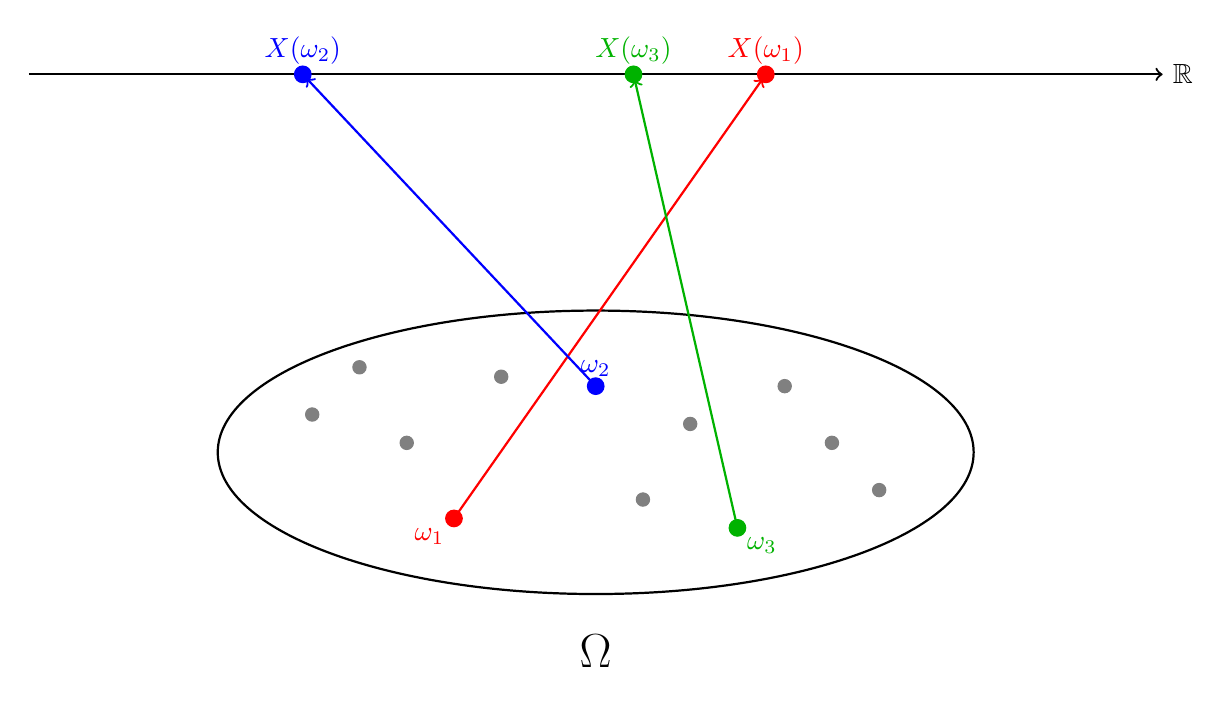
\begin{tikzpicture}[scale=1.2]
		
		% Flèche horizontale pour les réels
		\draw[->, thick] (-6, 4) -- (6, 4) node[anchor=west] {$\mathbb{R}$};
		
		% Ellipse avec label Omega (extérieur, en bas, très grand)
		\draw[thick] (0, 0) ellipse (4 and 1.5);
		\node at (0, -2.1) {\LARGE $\Omega$};
		
		% Points anonymes
		\foreach \x/\y in {
			-3/0.4, -2.5/0.9, -2/0.1, -1/0.8,
			0.5/-0.5, 1/0.3, 2/0.7, 2.5/0.1, 3/-0.4
		}{
			\filldraw[gray] (\x,\y) circle (2pt);
		}
		
		% Points étiquetés colorés comme flèches
		\filldraw[red] (-1.5,-0.7) circle (2.5pt) node[below left] {$\omega_1$};
		\filldraw[blue] (0,0.7) circle (2.5pt) node[above] {$\omega_2$};
		\filldraw[green!70!black] (1.5,-0.8) circle (2.5pt) node[below right] {$\omega_3$};
		
		% Points sur R (valeurs) colorés aussi
		\filldraw[blue] (-3.1, 4) circle (2.5pt) node[above] {$X(\omega_{2})$};
		\filldraw[red] (1.8, 4) circle (2.5pt) node[above] {$X(\omega_{1})$};
		\filldraw[green!70!black] (0.4, 4) circle (2.5pt) node[above] {$X(\omega_{3})$};
		
		% Flèches colorées, raccourcies avant les points (avec shorten >=)
		\draw[->, thick, red, shorten >=2pt] (-1.5,-0.7) -- (1.8,4);
		\draw[->, thick, blue, shorten >=2pt] (0,0.7) -- (-3.1,4);
		\draw[->, thick, green!70!black, shorten >=2pt] (1.5,-0.8) -- (0.4,4);
		
	\end{tikzpicture}
	
\end{document}
